\documentclass[a4paper, 12pt, oneside]{book}
\usepackage[english]{babel} % choose the language
\usepackage[utf8]{inputenc} % åäö
\usepackage[T1]{fontenc}
\usepackage[a4paper, inner=3cm, outer=3cm, top=3cm, bottom=3cm]{geometry}
\usepackage[onehalfspacing]{setspace} 
\usepackage{float}
\usepackage{mathptmx} % Times New Roman
\usepackage{tikz} % Support for pictures in latex format -> convert svg files into tikz format at first
\usepackage{amsfonts}
\usepackage[toc,page]{appendix}
\usepackage{etoolbox} % this one makes a workaround with page numbering possible
\usepackage{subfig}
\usepackage{csquotes} % BibLaTex stuff
\usepackage[toc, page]{appendix}
\usepackage{geometry}
 \geometry{
 a4paper,
 total={170mm,257mm},
 left=40mm,
 top=25mm,
 }

% Table of contents
\setcounter{secnumdepth}{5}
\setcounter{tocdepth}{5}

\begin{document}

\pagestyle{empty}    
\begingroup
\patchcmd{\chapter}{plain}{empty}{}{}

%------ Cover page stuff 

\begin{titlepage}
\vspace*{144pt}
\begin{center}
\Huge\bf The analysis and preprocessing of raman spectra of glioma cells %------ NAME OF THE THESIS HERE!!!


\end{center}
\enlargethispage{3cm}
\vfill

\hfill
\begin{tabular}[t]{l@{}}%{\raggedleft%
\textit{Author:} Joel Sjöberg 38686\\ % YOUR NAME AND STUDENT ID!
Masters thesis in Computer Science\\ % BAC/MASTER THESIS AND MAIN SUBJECT
\textit{Supervisor:} Luigia Petre\\ % NAME OF YOUR SUPERVISOR
The Faculty Of Science And Engineering\\ % FACULTY
Åbo Akademi University\\ 
2021\\ % YEAR
\\
\\
\\
\\
\end{tabular}
%}%
\end{titlepage}

%------ end of cover page stuff

\tableofcontents 


\endgroup % end of TeX group

\clearpage
\pagestyle{plain}      
\pagenumbering{arabic} % Page numbering starts from here
% Example of structure
\chapter*{Foreword}
\title{Foreword}

Backword
\\

Through what feels like uncountable hours in a hunchback-like state which could only be provoked by the most wholesome of encouragement I managed to produce this thesis(or, the thesis thus far). Remember Hofstadters law: "It always takes longer than you expect, escpecially when you take into account Hofstadters law".
Thank you to fellow:  \textbf{Fellow0, Fellow1, Fellow2, Fellow3, ..., FellowN} where N -> $\infty$

\chapter*{Abstract}
\title{Abstract}

Glioma is a cancer which begins in the glial cells within the brain. The presence of glioma tumors within the brain can cause a wide variety of symptoms, e.g. seizures, headaches and nausea. The analysis of these tumors is a long and tedious process yet it is essential in determining the correct line of treatment for patients whose life expectancy ranges between a couple of years to a matter of months. Optimizing the process of diagnosing these tumors is of great interest to the medical field. Furthermore, recent studies presents new ways of categorizing these tumors by analyzing the methylation type rather than grade and glial cell of origin. A possible way of analyzing glioma tumors is found through the use of Raman spectroscopy. The Raman spectra of the tumors contain information about the vibrations within the molecules of the tumor material.

Machine learning is a technique which has helped in analyzing non-trivial patterns  and automating tasks previously thought impossible to perform with computers. The technique utilizes data to form models which have been successful to the point of outperforming their human counterparts. It is evident that the models can perform well in situations where tremendous amounts of data is available. Within cancer research, the focus is on qualitative data gathering rather than quantitative. This because data gathering is often expensive and lacking due to a limited number of patients available for study.  

In this thesis, we explain the process of analyzing the spectra extracted from the tumors of glioma patients. The analysis is performed by sorting the spectra into different groups which maintain minimal variance among the different frequencies within the grouped spectra. This is done to separate tumor spectra from spectra extracted from non-tumor material which may have been present during scanning i.e. plastic, blood, necrotic tissue etc. We utilize machine learning methods to group and examine the samples in detail. We also validate the analysis and pre-processing by creating a model in attempt to classify the tumors according to the new categories based on the methylation types. Our findings and conclusions as to how these methods can be utilized further for improved results are also presented as conclusion in this thesis.  



%\chapter{Introduction}
%
\title{Motivation}

Please!! \cite{test}


\bibstyle{biblatex}
\bibdata{referenser,bib}
\citation{biblatex-control}

\chapter{Introduction}
The mammalian brain contains so-called neurons and glial cells. Historically it was believed that the brain contained ten times more glial cells than neurons, but recent studies suggest the number of neurons are equal to the number of glial cells \cite{von2016search}. Glial cells were previously thought to be insignificant in terms of the brains computational functionality, only lending structural support to the neurons. Recent studies have disputed this and suggest their contribution to the nervous system is greater than once thought, though their actual function is still a matter of speculation. Glioma is a type of brain cancer which manifests within the glial cells and disrupts brain functions. The survivability of the cancer is extremely poor with a life expectancy of a few months without treatment to a few years depending on the patients health, the tumor type and grade; rarely do patients survive for five years \cite{glialcells, gallego2015nonsurgical, bleeker2012recent}. Gliomas are categorized depending on their glial-cell of origin. There are four main types of glial cells (also called neuroglia or simply glia): oligodendrocytes, astocytes, ependymal cells and microglia. Oligendroglioma originates from oligodendrocytes, astocytoma from astocytes and ependymomas originate from ependymal cells. Furthermore, astocytoma-types may develop into glioblastoma multiforme (GBM), the most aggressive form of brain cancer; this may even communicate with  microglia to increase tumor growth \cite{maas2020glioblastoma}. It is also possible for GBM to develop from other brain cells \cite{glialcells}. This cancer is particularly aggressive due to its quick reappearance in the brain only a short period after surgery \cite{gallego2015nonsurgical}. The heterogeneity of GBM-cells further complicates the healing process, due to poor response to targeted treatments \cite{dirkse2019stem}.

The World Health Organization (WHO) has defined four levels (or "grades") of cancer severity used to describe the cancer aggressiveness and tumor growth. Grades I and II are considered low-grade and grades III and IV are considered high-grade. Glioblastoma is cathegorized as a grade IV cancer \cite{bleeker2012recent, gradesandpriorsubdivision}; these grades are used to determine an appropriate prognosis and line of treatment. A study by Vigneswaran et al. \cite{gradesandpriorsubdivision} suggested these grades could be divided further to better describe the features of the tumor and express versions with poor prognosis. This suggestion is also supported by Hirose et al. \cite{hirose2013subgrouping}. Ceccarelli et al. \cite{cellsubsets} introduce alternative subdivisions of these classes, which show promise in expanding knowledge about glioma tumors and aid in treatment selection. Such evaluations require in-depth knowledge about the tumor tissue and further examination, which may last for weeks after extraction. Ceccarelli et al. define the subdivisions by six distinct classes, labeled LGm1-6. Their analysis showed IDH mutations in LGm1-3, as the name suggests, IDH mutations refers to mutations in the IDH1 or IDH2 genes whihc encode for the enzymes IDH1 and IDH2. These mutations are shown to be significant in a variety of cancers, including glioma \cite{dang2016idh}. Furthermore, LGm4-6 were IDH wild-type, where a majority of tumors could be labeled as glioblastoma. IDH wild-type refers to IDH genes with no mutations, but they are often correlated with poor prognosis in high-grade glioma. These clusters are reinforced by the results produced by Vigneswaran et al. The process of determining a prognosis and a line of treatment has great promise in improving patient outcome and is essentially influenced by classifying tumors into these subdivisions.

This thesis is the result of a project whose purpose is to optimize the categorization process, based on a deep learning model capable of predicting tumor-types in a matter of minutes. The project relies on tissue from tumors extracted from 45 patients and scanned using Raman spectroscopy. Raman spectroscopy was invented by Chandrasekhara Venkata Raman and measures the vibrations of molecules by spectral analysis. This method can be executed fairly quickly and can provide chemical information from the spectral light. A laser emits a ray unto the tumor tissue, causing the energy level of the molecules within to change, which in turn changes their vibration. This vibration is gathered by the instrument and provides information regarding the molecular properties of the material \cite{long1977raman, graves1989practical}. This spectra is the data which the model uses as training and testing data. The choice of using Raman spectra in this way is due to the method's success in previous studies of Raman spectra using machine learning \cite{ramanDL, ho2019rapid}. The use of Raman spectra is further motivated by Liu et al. \cite{liu2017deep}, whose work show promise for deep learning models trained on raw Raman spectra. The advantage of this method in the context of multilabel classification seem considerable, when compared to other machine learning methods such as Support Vector Machines, Random Forest and K-nearest neighbor \cite{liu2017deep}.

This thesis aims to analyze the spectra extracted from all patient samples in an attempt to automate outlier detection. The samples are examined by statistical methods designed specifically for that purpose. Hierarchical clustering and K-means clustering are applied to the samples to divide the spectra into subsets which we find identifies many outliers. These results are examined in contrast to the results of a criterion for finding outliers in the data by the provider, after which the method most suitable for his purpose is used to remove the outliers. Following the removal of the outliers, we present a preprocessing pipeline which will be used to prepare the data for machine learning applications such as Artificial Neural Networks or Support Vector Machines. The features which best divide the data into the six LGm classes are extracted using f-classif. These features drastically reduces the size of the spectra which are analyzed for prognosis which in turn reduces the examination time. The thesis then aims to provide a clear way of preparing Raman spectra for machine learning applications and provides the most important features those spectra consist of. Suggestions and a discussion for how these methods may be improved, which alternative methods could be tested instead and eventual limits to this project are also given for future consideration.

The thesis is structured as follows, Chapter 2 presents the preliminary  background for the statistical methods used in the project, along with the necessary mathematical definitions by which these methods are defined. Among these are the notion of the mean and standard deviation which are central to methods of analysis we use, this includes the analysis of variance (ANOVA) which is applied by the f-classif method for extracting features from the data. Understanding the underlying definitions and consequences is necessary to validate and confirm the results and as such, the chapter also presents the definition of supervised and unsupervised learning with short definitions on machine learning terminologies. The formal definitions of K-means clustering and Hierarchical clustering is given. In Chapter 3, we discuss the exploration methods in detail, to give further understanding of the data on which this project is based. The chapter begins by introducing the concrete shape of the data. Feature selection is applied to the data by the f-classif method and the results are examined. The majority of this chapter is based on the visual analysis of the outlier detection. This is done by applying the statistical methods and the clustering methods to the samples. The results of each method are analyzed in contrast to the criterion defined by the dataprovider in greater detail to form an argument for or against the method in question. The chapter ends by removing the outliers by the optimal method and performing feature selection once more on the data devoid of outliers. In Chapter 4, we present our suggestion as well as arguments for the preprocessing pipeline to prepare the data for machine learning. An Artificial Neural Network is created and trained on the curated data. The performance of the architecture is measured and presented. The thesis is concluded in Chapter 5, where we discuss improvements and suggestions to out methods. We also provide suggestions for alternative methods used for feature selection and preprocessing for future study and tests. % chapters actually begins from 2, motivation is chapter 1

\chapter{Theoretical Background}
In this chapter we present the necessary mathematical concepts on which this thesis is based. The concepts are considered fundamental for understanding the methods applied in the project. It begins by 
covering necessary mathematical theory required to understand data representations and handling within Machine Learning (ML). It then proceeds by defining common concepts in machine learning and the subject of supervised and unsupervised learning.


\section{Mathematical Foundations}

\section{Machine Learning}

Machine learning is the practice of computing models for relationships between sets of data. The field has garnered significant interest within academia and industry alike due to the promising result in applications for which deterministic algorithms have proven difficult or impossible to make. There are two paradigms for learning: Supervised learning (using labeled data to approximate models) and unsupervised learning (finding patterns within the data itself). 

Models are used to great length within many scientific domains. Though each domain has defined this term differently, the definitions in the context of machine learning shall be used. In this context, a model is a data structure made out of constant parameters which may be performed on any input vector $x$ to produce a prediction $y$

\vspace{5mm}

\textbf{Definition: } A model is an approximation of a desired function $f$ which produces relevant results based on human definitions.  

\vspace{5mm}

Mathematically a model may be represented as a collection of numbers $M$ which may in turn be used to compute $f$ for any given example.
In the context of machine learning a set of parameters may be tuned during a learning process (or training process). These parameters are combined with samples of data through some mathematical procedure to effectively model a distribution from which the data was extracted. The equation below is an example of a n-dimensional object.
$$x_0\theta_0 + x_1\theta_1 + ... + x_n\theta_n$$

\subsection{K-means Clustering}

Clustering is an unsupervised learning method whose primary use is in grouping sets of data. In this thesis we consider the \textit{K-means clustering} algorithm. The following is a formal definition of \textit{K - means clustering} as defined by MacQueen \cite{macqueen}. Given a set of $N$-dimensional points (where $N \in \mathbb{N}$) $E_N$ and a desired amount of partitions $k$ of $E_N$, partition the elements of $E_N$ into $k$ sets $S = \{S_1, S_2, ... S_k\}$. The partitioning of $E_N$ is performed by randomly initializing $k$  $N$-dimensional points as randomly selected points within $E_N$. We define the set $V$ with elements $v$ where $v_i$ is the i:th cluster center where $i \in [0, k]$. The partitioning of the elements $x \in E_N$ into their respective partition $S_i$ is performed by computing the closest cluster center $\forall_{x \in E_N}$. Let $T_i$ be the set of $x \in E_N$ such that the distance from the element to the relevant cluster is minimal, $T_i$ is defined by formula \ref{eqn:Ti}.

\begin{equation}
\label{eqn:Ti}
T_i = \{x : x \in E_N | (\forall_{j \in [0, k]/i } |x - v_i| \leq |x - v_j|)\} 
\end{equation}

For centers who share equal distance to any given $x$ the cluster with the smallest index is chosen as the containing set. The partitions $S_i \in S$ are defined by formula \ref{eqn:Si}

\begin{equation}
\label{eqn:Si}
S_i = T_i \cap \bigcap_{j=0}^{(i-1)} S_j^c
\end{equation}

A consequence to this definition is that outliers have a potential to drastically change the quality of the cluster outcomes\cite{chawla2013k}. To remedy this and the stochastic nature of the initialization process, the method is run several times on the same dataset, yielding the resulting clusters with minimal inertia. The problem \textit{K-means clustering} attempts to solve is proven to be NP-hard\cite{chawla2013k}\cite{mahajan2009planar} but the algorithm itself has a time complexity of $O(n^2)$\cite{pakhira2014linear}.


\subsection{Hierarchical clustering}

Hierarchical clustering is a clustering method which has a deterministic process. Each cluster formed is based on the entire dataset in contrast to \textit{K-means} which approximates clusters by performing small changes to the cluster centers. The method produces clusters by iteratively combining the closest clusters according to the given linkage criterion (defined in the sections below). The two primary strategies for forming clusters are \textit{agglomerative} and \textit{divisive}. Agglomerative clustering initializes one cluster for each data point and combines them in a hierarchy according to the linkage criterion until all clusters are part of the hierarchy. Divisive strategies initializes one universal cluster for all data points and proceeds to separate the points into distinct clusters according to the linkage criterion. The method proceeds until all data points are separated to their own cluster within the unifying hierarchy. The project described in this thesis uses the \textit{agglomerative} strategy. All strategies depend on the distance measure and linkage criterion \cite{murtagh1983survey}.

\subsubsection{Distance metrics}
Let $u$ and $v$ be vectors of the same dimension $n$. The \textit{Euclidean distance} (also called \textit{L2-distance}) measure can be used to measure distance between the vectors in euclidean space. The \textit{Euclidean distance} is calculated by equation (\ref{eqn:euclid}).

\begin{equation}
\label{eqn:euclid}
d(u, v) = \sqrt{\Sigma_i (u_i - v_i)^2} 
\end{equation}

The \textit{Manhattan distance} (also called \textit{L1-distance}) metric is also a viable alternative if the distance is to be measured in blocks. The distance is akin to finding a shortest path among blocks and is therefore calculated as expressed in equation (\ref{eqn:manhattan}).

\begin{equation}
\label{eqn:manhattan}
d(u, v) = \Sigma_i |u_i - v_i|
\end{equation}

\textit{Cosine similarity} measures similarity between vector angles and suits situations where certain vectors are expected to be similar. Should the vectors be sizable in terms of dimensionality, this method will yield varying results, especially if the elements have significant variance in each dimension. It is calculated as expressed in equation (\ref{eqn:cosine}).

\begin{equation}
\label{eqn:cosine}
d(u, v) = \frac{\Sigma_i u_iv_i}{\sqrt{\Sigma_i u_i^2}\sqrt{\Sigma_i v_i^2}}
\end{equation}

\subsubsection{Linkage Criteria}
In order to measure distance between clusters it is essential to know between which points the distance should be measured, since clusters often consist of several points. Linkage criteria describes the method for determining how the distance metric will be applied. SKlearn define four criteria in the documentation \cite{scikit}: Single linkage, complete linkage, average linkage and ward linkage. Depending on which criterion is applied the results may differ considerably, it is therefore vital to have a formal understanding of their application and consequences.

Single linkage goes through each pair of clusters measuring the distance among all points within one with respect to the other. The distance between these clusters is determined to be the distance between the two closest points. Let $U$ be the elements in the first cluster and $V$ be the elements of the second. The distance between the first and the second cluster is defined formally in equation (\ref{eqn:single}).

\begin{equation}
\label{eqn:single}
d(U, V) = \forall_{u, v \in U, V} min(d(u, v))
\end{equation}

Single linkage tend to produce trivial results, forging a hierarchy in a chain where individual elements slowly merge with the bigger cluster. In contrast complete linkage considers the largest distance between two points for every pair of clusters. The distance between two clusters then become the distance between the points which are the furthest apart. Formally expressed in equation (\ref{eqn:complete}).

\begin{equation}
\label{eqn:complete}
d(U, V) = \forall_{u, v \in U, V} max(d(u, v))
\end{equation}

By considering the largest possible distance between two clusters it bypasses the setback by single linkage, allowing more clusters to form before merging into one unifying cluster. Average linkage calculates the average between all elements for every pair of clusters and merges the ones possessing to the minimal average distance. Formally described by equation \ref{eqn:average}.

\begin{equation}
\label{eqn:average}
d(U, V) = \frac{1}{|U||V|}\sum\limits_u^U \sum\limits_v^V  d(U_u, V_v)
\end{equation}

Ward linkage represents distance by how much the summed square would increase by merging them. The method aims to merge the clusters such that the within cluster variance is minimal. Let $c_a$ be the center of cluster a, then ward linkage is expressed formally by equation \ref{eqn:ward}\cite{shalizi2009distances}.


\begin{equation}
\label{eqn:ward}
d(U, V) = \frac{|U||V|}{|U|-|V|}||c_U - c_V||^2
\end{equation}



\subsection{Feature Selection}

In many cases the data available contains numerous features, which often helps to building sufficient classifiers as the model may find non-trivial patterns among the features. To avoid expanding the dependence on large datasets, it is often necessary to strip the data of certain features which possess minimal correlation to other features or which lack that correlation entirely \cite{dash1997feature}. Features that possess the necessary expressive information are not always trivial, there are several ways in which they may be found. \textbf{TODO: Expand this, it's been 3 weeks already!}

\section{Deep Learning}

The field of Artificial Intelligence is founded on the notion of designing algorithms for solving problems. The field encountered tremendous progress in \textbf{[FIND YEAR, AI FOUNDATIONS]} referred to by \textbf{[NAME]} as the "look ma, no hands" era of Artificial Intelligence. One such method which have proven useful for these tasks is the practice of approximating models through Artificial Neural Networks.

\subsection{Artificial Neural Networks}
Artificial Neural Networks ("ANNs") have been used to great success during the 20th century [\textbf{Source Here}]. With the use of ANNs
several fields including Natural Language Processing, Encoding and Image classification have undergone revolutionary leaps in performance regarding optimization due to the predictive power of these networks [\textbf{Source Here}]. At the same time they are heavily criticized for their complexity, yielding a structure much more akin to a so called \textit{"black box"} than a reliable and deterministic method for prediction[\textbf{Source Here}]. This complexity is due to numerous different structural typologies available at present and an awesome number of tuned parameters which are modified with the goal of minimizing the predictive error [\textbf{Source Here}].

A consequence of this is hard skepticism in regards to the correctness of their functionality within practical use. While these models have shown great promise when compared to their human counterparts, the question remain whether or not perfect performance can be yielded from the constructed models.\\

\textbf{Definition 1.} Training an ANN is allowing minuscule changes through the randomly initialized structure in order to approximate a collection of nested functions $$f_n(f_{n-1}(...f_1(X)))$$ 

\subsection{Computational Representations}
The initial purpose of ANNs was to create a computational model of the human cortex which took the form of the McCulloch, Pitts neuron. The multilayer perceptron (MLP) introduced in \textbf{[year here]} formed the basic structure which would become ANNs. 


 

\chapter{Data Exploration}
Deep learning models require tremendous amounts of data, to ensure the model works well the data must also possess sufficient characteristics to approximate the sample population from which it was extracted. To satisfy this requirement we examine the data in attempt to remove outliers and determine whether the data is sufficient for classification. Moreover, certain tumors may be heterogeneous \cite{friedmann2014glioblastoma}, which may be problematic for a classifier as heterogeneous samples lack in shared characteristics. In this chapter the data available to the project is examined in greater detail; details for how the Raman spectra were prepared is given to document the preprocessing of spectra for future use. First we describe the mathematical representation of the samples. Since the number of samples is too small to use in a deep learning model, we explain how each sample may be separated into individual spectra; this separation yields a drastic increase in the number of available training examples. We then explain how to balance the data; an unbalanced dataset would likely introduce bias in the deep learning model, rendering its desired predictive capabilities uncertain. We achieve this by duplicating underrepresented samples-classes in the dataset. Furthermore, this balancing is performed to maintain majority and minority classes, thus retaining some distributional information from the original dataset. The quintessential purpose of this chapter is to analyze the data using k-means clustering and hierarchical clustering for detecting non-tumor spectra or otherwise erroneous spectra. These methods are tested in contrast to other outlier detection techniques such as the standard deviation test and the interquartile range method. Adrian's criterion is presented and compared to the the spectral images extracted from the samples.
Another point of interest in this project is the identification of representative frequencies within the spectra. Each spectra belongs to a tumor which can be categorized by six different classes. The hypothesis states certain frequencies should be sufficient in determining which class the tumor belongs to. For this feature selection is used, representing each frequency within the spectra as distinct features. This task is simplified by the new representation of the data separated into lists of spectra rather than a collection of spectra represented by the tumor. However in order to extract such features the data must be devoid of outliers. Should outliers exist within the dataset, the features given by the methods used will be influenced and may yield conflicting results with the ground truth. To prepare for this the data is plotted for visual inspection using various methods to be discussed in the following section on feature selection. It is confirmed by the provider that the majority of samples include faulty spectra e.g. spectra of blood drops on the sample or plastic which may be reflected form underneath thin tissue. Furthermore some tissue may be necrotic which will affect the spectral signal. Using the extracted features a model can potentially form around the data faster which can be essential as deep learning training require significant computing resources. The features are extracted before and after the removal of problematic spectra for comparison.


\section{Data Representation}
The data consists of the Raman-spectra extracted from the tissue of glioma tumors from 45 patients. Multiple samples of tissue were extracted from the same patient in some cases, yielding several samples for the respective patient. To maintain separation among the patients, the samples are sorted by their respective patient of origin. This is necessary, since there is uncertainty regarding the homogeneity among patient samples. The data will be separated into three separate datasets. These sets are called training set, validation set and testing set. All datasets will consist of unique patients to avoid scenarios in which the model overfits to a patients tumor sample and as a result of heterogeneity. This structure also allows for easier handling of the number of patients in the sample-classes, allowing for analysis on each class exclusively. 

There is also large variation with regard to the sample shape within the data. Each sample is a 3-dimensional array of shape $(w, h, 1738)$ where $w$ and $h$ are the width and height of the sample, respectively. This formalization is necessary, as width and height have non-zero variance among different samples. The shape is a result of how the tissue was scanned. In each case the tissue was placed inside the instrument and scanned successively from side to side. This makes it possible to display each sample as an image, by substituting the third dimension (denoted above by $1738$) a color value denoted by which class the spectra belongs to. The number $1738$ is constant through all samples and represents the length of a modified Raman-spectra which is performed by the provider, each element a unique frequency. Furthermore each element inside these arrays is a real number without clear bounds. The largest absolute element found within the complete dataset is $79427.0625$, some values are negative which is confirmed by the providers to have significance for the projects purpose. The project aims to predict which subdivision the spectra belong to by feeding in one of these samples, i.e., one vector of shape $(1, 1738)$. This strategy is inspired by Liu et al.\cite{liu2017deep}, who managed to get satisfactory performance by training a model on raw spectra. This representation is of great interest, since the value of each spectrum is independent from the surrounding spectra. Separation at this level yields a dataset with more than $300,000$ datapoints, which better suits deep learning tasks.

 
To prepare for the project each samples spectra is collected and plotted in one single plot to compare spectral information from the sample itself. An example of such plots can be seen in Appendix \ref{appendix:spectraplot}. Patient HF-1887 is removed from the project completely due to the skewed baseline in the spectra.


\section{Data preparation}
In this section we explain our qualitative analysis on the data, done to determine the plausibility of our model. Each sample is categorized according to their subdivision; there are six distinct subdivisions as defined by Ceccarelli et al. \cite{cellsubsets}, denoted LGm1 - 6. As an initial step each samples spectra is analyzed by visual inspection. The spectra are plotted on a two dimensional surface as lines, each line a unique spectrum. Through this analysis one sample is discarded due to the tilted baseline of the spectra, none of the other samples share this problem. A sample which shares a general shape with the other samples is shown in contrast to the sample selected for removal in \ref{appendix:spectraplot}. Another sample shows a concerning number of spikes in contrast to the other samples. The number of spectra is also considerably larger compared to the others, which is limiting for some of the methods selected for the analysis. For this reason the sample is also discarded.

\subsection{Organization and Balance}
The model will as a consequence of it's learning-algorithm become biased towards certain predictions. This because as the model encounters frequent examples of a certain class, the connections which produce such predictions will strengthen. Over exposure to examples of a certain class will force the model to associate features with that class, redirecting focus from classes for which that feature could be significant. The initial data suffers heavily from this problem, a is shown in Table \ref{table:1}.

\newpage

\begin{table}[h!]
\centering
 \begin{tabular}{||c c c c c c c||} 
 \hline
 Class & LGm1 & LGm2 & LGm3 & LGm4 & LGm5 & LGm6 \\ [0.5ex] 
 \hline\hline
 \# of samples & 5& 11 & 4 & 10 & 11 & 4 \\ 
 \hline
 \# of spectra & 37319 & 71846 & 31931 & 50660 & 62256 & 20176 \\
 \hline
 percentage & 14\%& 26\% & 12\% & 18\% & 23\% & 7\% \\
 \hline

\end{tabular}
\caption{Table showing the distribution of data in the initial dataset after removing the problematic samples. The number of samples are displayed on the first row, the number of spectra in each class is shown on the second row. The percentage of the entire dataset is shown on the third row. The majority class is LGm 2 and minority is LGm 6.  Classes LGm 1, 3 and 6 must be expanded to balance the data.}
\label{table:1}
\end{table}

Table \ref{table:1} shows the per class separation in the data, the header row shows the labels of each class. The first row shows the number of samples belonging to each class, these are the tumors which will be analyzed. The second row displays the total number of spectra across each class; these must be considered for balancing. Note the equal amount of samples in LGm3 and LGm6, but the difference in number of spectra within them. This is due to the varying size of all samples drawn from the tumors. Some samples share the same size, however the important fact is that the samples lack a uniform shape, which must be considered during the analysis. The last row shows the percentage each class makes of the entire dataset. Initially LGm2 is the majority class while LGm6 is the minority, consisting of only $7$\% of the entire dataset.

Before the data is balanced, the testing data is selected and separated from the rest manually. This is done by separating at least one patient and all their samples from the rest of the data. This way it will be possible to test if the model is develops bias towards the patients in training and if the patient samples are heterogeneous with respect to the other samples of the same class. The test-samples are chosen manually, samples are chosen with the criterion that approximately $30\%$ of each class is represented in the test set. Balancing the classes which contain less elements by a factor larger than or equal to two compared to the majority class (LGm2) is done by repeating the spectrum in each sample by that factor. Following this method the majority class will stay the majority which can be crucial provided the sample pattern is similar to the set of all other unseen samples. The resulting dataset is gained by doubling the samples in LGm1, tripling the samples in LGm3 and quadroupling the samples in LGm6. The distributions of the training dataset is shown in Table \ref{table:2}.
\\
\\
\begin{table}[htb]
\centering
 \begin{tabular}{||c c c c c c c||} 
 \hline
 Class & LGm1 & LGm2 & LGm3 & LGm4 & LGm5 & LGm6 \\ [0.5ex] 
 \hline\hline
 \# train & 21289	& 51698	& 20635	& 34276	& 37492	& 12976 \\
 \hline 
 \# test & 14945 & 20140 & 11296 & 16384 & 24764 & 7200 \\
 \hline

\end{tabular}
\caption{Distribution of the training data and the testing data}
\label{table:2}
\end{table}

Table \ref{table:3} shows the distribution of the training data and testing-data. The training data is then balanced exclusively. This is not required in the testing data, since it will have no effect on how the model is developed through training. The training data is balanced by replicating each spectra in every patient of the classes which are under-represented. The resulting training-set is gained by doubling the spectra in LGm 1 and LGM 3 and  the spectra in LGm 6. The final distribution of the training data following this procedure is shown in table \ref{table:3}

\begin{table}[htb]
\centering
 \begin{tabular}{||c c c c c c c||} 
 \hline
 Class & LGm1 & LGm2 & LGm3 & LGm4 & LGm5 & LGm6 \\ [0.5ex] 
 \hline\hline
 \# train & 42578 & 51698 & 41270 & 34276 & 37492 & 38928 \\
 \hline 

\end{tabular}
\caption{Distribution of the testing data following balancing}
\label{table:3}
\end{table}

\section{Analysis}

Following the balancing, the first step in the analysis is to get the frequencies which best describe the data with respect to the methylation-types. Each number in the spectra is a frequency at which the scattered light is gathered. This light is expected to be sufficient for predicting the methylation-type of the tumor-tissue. It is speculated that to sufficiently categorize the spectra into the methylation-types only certain frequencies are required. For this reason the best features are extracted with SelectKBestfeatures \cite{scikit} which is given the f-classif method for ranking the features which yields features deemed significant by ANOVA. The 70 best features were extracted from the training-data in which there are spectra which originate from non-tumor tissue. The features are displayed in Appendix \ref{appendix:features0}. Before the features are extracted, each spectra is standardized using z-score standardization, to give each spectrum a mean of zero and a standard deviation of one. This is done for ease of comparison among the spectra. The extracted features show that regions of interest do exist on the spectra. This can be seen by the integers which have a difference of one, suggesting that the region of interest exist somewhere in specific parts of the spectra. It is worth noting here that the features selected might be correct provided the amount of non-tumor spectra is sufficiently small to be ignored by the feature selection method. Due to this uncertainty, the data will be separated from the outliers and feature selection will be performed a second time.

To avoid bias the analysis is performed on the training data exclusively. The goal of the analysis is to find a uniform criterion which each spectrum must fulfill to be considered clean. Spectra which fail to satisfy this criterion will be discarded form the project entirely. In this section the methods of analysis used are described and their results examined, the section begins by examining the standard deviation test and interquartile range method, these are deterministic methods that rely solely on the values found within the data. k-means clustering and agglomerative clustering are then performed on the data in attempt to capture potentially complex patterns within the data. The section ends by presenting Adrians criterion, which is a criterion for finding problematic spectra defined by the data provider. 

\subsection{The standard deviation test}

The standard deviation test is a test by which the data is centered around the mean and given a standard deviation of one. With this setup outliers are defined as points which is separated from the mean by 3 standard deviations or more. As the spectral information might differ among patients, the test is performed on each tumor separately. From each tumor, the mean and standard deviation is calculated from each frequency. The values are then used to standardize each spectra belonging to the tumor. A spectra is deemed to be an outlier if the 

\subsection{Old text}
To ensure each sample include relevant information requires intuitive analysis. During extraction it is possible droplets of non-tumor material was present e.g. blood or lipids, it is also possible the laser hit the tissue at a thin point which would scan the plastic underneath. This data must be removed to avoid model dependency on erroneous spectra. To find and remove the erroneous spectra, a clustering method is used. A suggested method is the k-means clustering algorithm by MacQueen \cite{macqueen} performed on every spectra on a sample by sample analysis. The resulting clustering may be displayed as a 2-dimensional image, some of which are shown in \textbf{APPENDIX!!}. K-means do however suffer heavily from outlier influences, as these outliers may be present at this stage, it is necessary to consider other methods. Hierarchical clustering is a clustering method which avoids outlier dependency by separating each individual spectra into its own cluster and then reducing the number of clusters depending on the linkage type. Complete linkage is used to ensure diversity among the clusters, measured by euclidean distance\cite{scikit}. Each spectra is now labeled by a class number, all labels may be displayed as a two dimensional image due to the shape of the samples. Examples of such images are shown in appendix \ref{appendix:hierimg0}. The cluster shapes suggest certain outliers within all patients, these outliers are removed accordingly to retain the tissue information exclusively.

\subsection{Feature selection (OLD)}


Each number in the spectra is a frequency at which the scattered light is gathered. This light is expected to be sufficient for predicting the methylation-type of the tumor-tissue. Due to the number of spectra inside each sample memory quickly becomes an issue, it is therefore relevant to examine which frequencies would have the most impact on classification. For this reason the best features are extracted with SelectKBestfeatures \cite{scikit}. The 70 best features were extracted from each spectra which is shown to be appropriate to recreate the original tumorshape by performing clustering 

\chapter{Results}

\chapter{Conclusion}

\bibliographystyle{ieeetr}
\bibliography{ref}% ref.bib


\begin{appendices}
\chapter{Spectral Plots}

\begin{figure}[h]
\label{appendix:spectraplot}
    \centering
    \subfloat[\centering Spectra from patient HF-1293. The rest of the samples available share in this pattern with some deviations]{{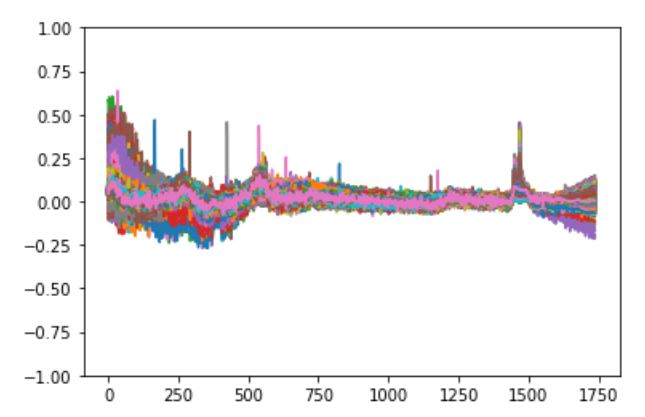
\includegraphics[width=5cm]{images/1293graph.JPG} }}
    \qquad
    \subfloat[\centering Spectra from patient HF-1887. The frequencies tilt towards the upper part of the plot. The example is decidedly removed from the analysis.]{{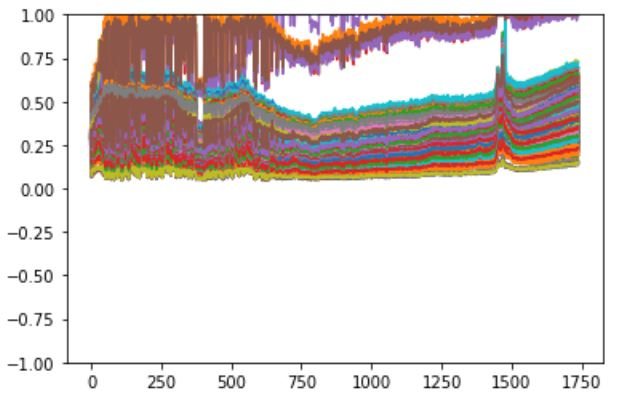
\includegraphics[width=5cm]{images/1887graph.JPG} }}%
    \caption{Examples of samples drawn from the data, HF-1293 display a common pattern across all samples, HF-1887 is removed due to problematic handling}%
\end{figure}

\chapter{Feature Selection}

\label{appendix:features0}
begin 250  309  522  523  524  525  526  527  528  529  553  563  645  646
  647  648 1450 1451 1452 1453 1454 1455 1456 1457 1458 1459 1460 1461
 1462 1463 1464 1465 1469 1470 1471 1472 1473 1474 1475 1476 1477 1478
 1479 1480 1481 1482 1483 1484 1485 1486 1487 1488 1489 1490 1491 1492
 1493 1494 1495 1496 1497 1498 1499 1500 1501 1502 1503 1511 1512 1513 end


\chapter{Spectral Images For Outlier Detection}

\end{appendices}

% Multiline command from stackexchange, hide this text
\newcommand{\comment}[1]{}
\comment{
\appendix
%\chapter{Appendix}

\begin{figure}[h]
\label{appendix:spectraplot}
    \centering
    \subfloat[\centering Spectra from patient HF-1293. The rest of the samples available share in this pattern with some deviations]{{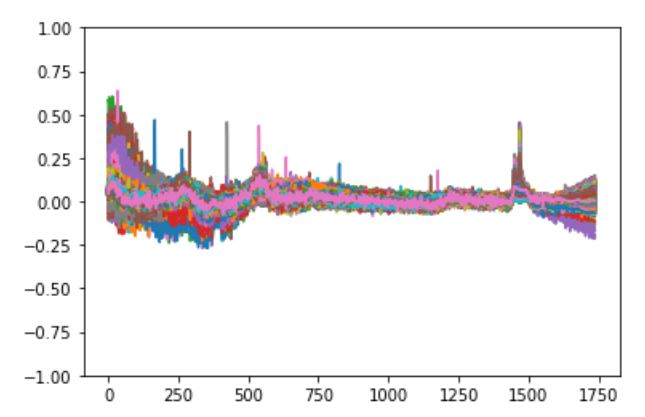
\includegraphics[width=5cm]{images/1293graph.JPG} }}
    \qquad
    \subfloat[\centering Spectra from patient HF-1887. The frequencies tilt towards the upper part of the plot. The example is decidedly removed from the analysis.]{{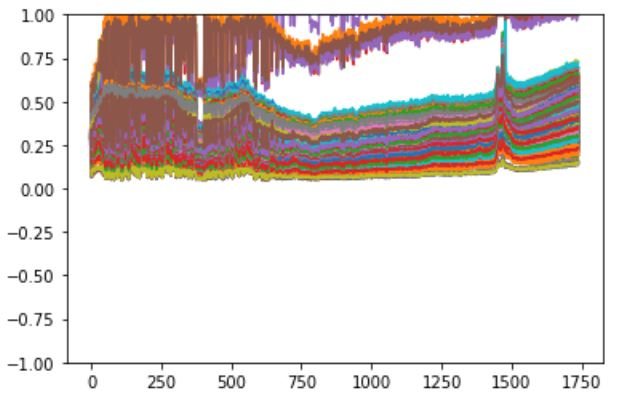
\includegraphics[width=5cm]{images/1887graph.JPG} }}%
    \caption{Examples of samples drawn from the data, HF-1293 display a common pattern across all samples, HF-1887 is removed due to problematic handling}%
\end{figure}


\label{appendix:features0}
begin 250  309  522  523  524  525  526  527  528  529  553  563  645  646
  647  648 1450 1451 1452 1453 1454 1455 1456 1457 1458 1459 1460 1461
 1462 1463 1464 1465 1469 1470 1471 1472 1473 1474 1475 1476 1477 1478
 1479 1480 1481 1482 1483 1484 1485 1486 1487 1488 1489 1490 1491 1492
 1493 1494 1495 1496 1497 1498 1499 1500 1501 1502 1503 1511 1512 1513 end

Adrians criterion concerns frequencies labeled by the features from 1463 to 1473. Almost all features are present, with the exception of features 1466, 1467 and 1468. 

\label{appendix:hierimg0}

}


\end{document}